\begin{surferPage}[Labs-Septic]{منحنى سباعي ذو 99 متفرداً}
      قام أوليفر لابس
      \textenglish{(Oliver Labs)}
       ببناء منحنى من الدرجة $7$ (سباعي) بينما كان يعمل على أطروحته في جامعة ماينتس في العام 2004. هذا هو الرقم القياسي الحالي للدرجة $7$. ولكن من المحتمل وجود منحنى سباعي يصل عدد متفرداته إلى $104$!
    يملك منحنى لابس تناظر مضلع سباعي منتظم (الصورة على اليسار). يمكن رؤية ذلك عند النظر إلى المنحنى من أعلى (الصورة على اليمين):

    \vspace*{-0.3em}
    \begin{center}
      \begin{tabular}{c@{\qquad}c}
        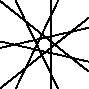
\includegraphics[height=1.5cm]{./../../common/images/labsseptic1.pdf}
        &
        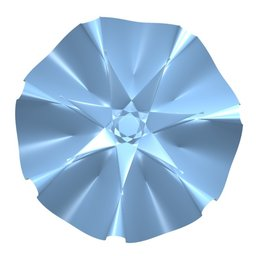
\includegraphics[height=1.5cm]{./../../common/images/labs_septic_von_oben}
      \end{tabular}
    \end{center}
    \vspace*{-0.3em}

    من أجل بناء هذا المنحنى، استعمل أوليفر لابس نظام الحساب الرمزي المحوسب سنغولار \textenglish{\sc Singular} (جامعة كايزرسلاوترن) الملائم تماماً للحسابات في مجال الهندسة الجبرية والمتفردات.

    إعتمد على امكانية الحسب مع مجموعة محدودة من الأرقام بطريقة طبيعية. نعرف هذا من حسابيات الساعة؛ 24.00$=$0.00, 24.00 $+$ 1 ساعة لا نحصل على 25.00 ولكن على 1.00.
\end{surferPage}
